%% \begin{frame}
%% 栈和队列是两种应用非常广泛的数据结构,它们来自线性表数据结构,都是“操作受限”的线性表。栈在计算机的实现有多种方式:
%% \begin{itemize}
%% \item[$\diamond$]硬堆栈
%% \item[] 利用CPU中的某些寄存器组或类似的硬件或使用内存的特殊区域来实现。这些堆栈容量有限,但速度很快。
%% \item[$\diamond$]软堆栈
%% \item[] 这类堆栈主要在内存中实现。堆栈容量可以达到很大,在实现方式上,又有动态方式和静态方式两种。
%% \end{itemize}•
%% \end{frame}

\section{栈}

\subsection{基本概念和抽象数据类型}
\begin{frame}\ft{\subsecname}
  \begin{dingyi}[栈]
    栈(Stack)是限定仅在表尾进行插入和删除操作的线性表。
  \end{dingyi}
  \begin{itemize}
  \item[$\diamond$] 允许进行插入、删除操作的一端称为栈顶(top),另一端称为栈底(bottom);\\[0.1in]
  \item[$\diamond$] 不含任何数据元素的栈称为空栈;\\[0.1in]
  \item[$\diamond$] 栈又称后进先出(Last In First out)的线性表,简称LIFO结构。
  \end{itemize}•

\end{frame}

\begin{frame}\ft{\subsecname}
  \begin{itemize}
  \item 栈是一种特殊的线性表,仍具有前驱后继关系。\\[0.1in]
  \item 栈限制了插入和删除的位置,这些操作始终只在栈顶进行。于是栈底是固定的,最先进栈的只能在栈底。
  \end{itemize}
\end{frame}
%

\begin{frame}\ft{\subsecname}
设栈$S=(a_1,a_2,\cd,a_n)$,称$a_1$为栈底元素,$a_n$为栈顶元素。

  \begin{figure}
  \centering
  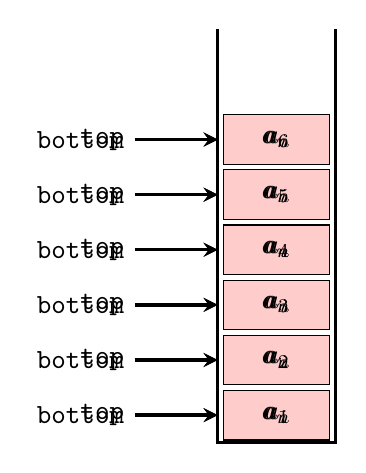
\begin{tikzpicture}
    \tikzstyle{information text}=[rounded corners,fill=blue!20,inner sep=1ex]
    \def\x{1.5}
    \def\y{0.7}
    \def\r{8}
        
    \draw[very thick] (\r,7.5*\y)--(\r,0*\y)--(\r+\x,0*\y)--(\r+\x,7.5*\y);
    
    \foreach \c in {1,2,...,6}{
      \filldraw[fill=red!40,fill opacity=0.5] (\r+0.05*\x,\c*\y-0.95*\y)rectangle(\r+0.95*\x,\c*\y-0.05*\y);
      \ifthenelse{\c=3 \OR \c=5}{
        \node [] at (\r+0.5*\x,\c*\y-0.5*\y) {$\cd$};
      }{
        \ifthenelse{\c=1 \OR \c=2}{
          \node [] at (\r+0.5*\x,\c*\y-0.5*\y) {$a_\c$};
          \ifthenelse{\c=1}{
            \draw[->,>=stealth,very thick] (\r-0.7*\x,\c*\y-0.5*\y) node[left] {\tt{bottom}}--(\r+0,\c*\y-0.5*\y);
          }{}
        }{
          \ifthenelse{4=\c }{
            \node [] at (\r+0.5*\x,\c*\y-0.5*\y) {$a_i$};
          }{
            \node [] at (\r+0.5*\x,\c*\y-0.5*\y) {$a_n$};
            \draw[->,>=stealth,very thick] (\r-0.7*\x,\c*\y-0.5*\y) node[left] {\tt{top}}--(\r+0,\c*\y-0.5*\y);
          }
        }
      }
    }
  \end{tikzpicture}
\end{figure}


\end{frame}
%
%
\begin{frame}\ft{\subsecname}
  \begin{itemize}
  \item 栈的插入操作叫做进栈,也称压栈、入栈。\\[0.1in]
  \item 栈的删除操作叫做出栈,也称弹栈。
  \end{itemize}
\end{frame}

\begin{frame}\ft{\subsecname}

  \begin{figure}
  \centering
  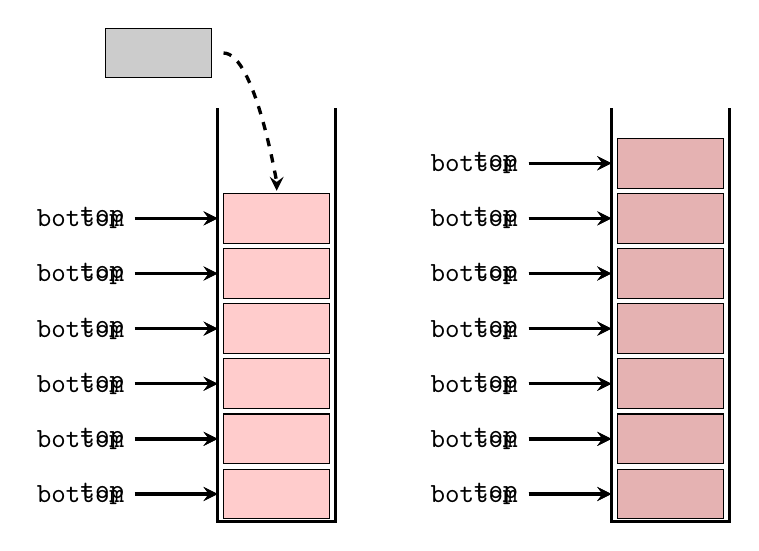
\begin{tikzpicture}
    \tikzstyle{information text}=[rounded corners,fill=blue!20,inner sep=1ex]

    \def\x{1.5}
    \def\y{0.7}
    \def\r{0.5}
    \def\c{9}
    
    \filldraw[fill=black!40,fill opacity=0.5] (\r+0.05*\x,\c*\y-0.95*\y)rectangle(\r+0.95*\x,\c*\y-0.05*\y); 
    \draw[->,>=stealth,dashed,very thick] (\r+1.05*\x,\c*\y-0.5*\y) .. controls +(right:4mm) and +(up:1mm) .. (2+0.5*\x,6*\y);

    \def\r{2}
    \draw[very thick] (\r,7.5*\y)--(\r,0*\y)--(\r+\x,0*\y)--(\r+\x,7.5*\y);
    \foreach \c in {1,2,...,6}{
      \filldraw[fill=red!40,fill opacity=0.5] (\r+0.05*\x,\c*\y-0.95*\y)rectangle(\r+0.95*\x,\c*\y-0.05*\y);
      \ifthenelse{\c=1}{
        \draw[->,>=stealth,very thick] (\r-0.7*\x,\c*\y-0.5*\y) node[left] {\tt{bottom}}--(\r+0,\c*\y-0.5*\y);
      }{}
      \ifthenelse{\c=6}{
        \draw[->,>=stealth,very thick] (\r-0.7*\x,\c*\y-0.5*\y) node[left] {\tt{top}}--(\r+0,\c*\y-0.5*\y);
      }{}
    }

    \pause 
    \def\r{7}
    \draw[very thick] (\r,7.5*\y)--(\r,0*\y)--(\r+\x,0*\y)--(\r+\x,7.5*\y);
    \foreach \c in {1,2,...,7}{
      \ifthenelse{\c=7}{
        \filldraw[fill=black!40,fill opacity=0.5] (\r+0.05*\x,\c*\y-0.95*\y)rectangle(\r+0.95*\x,\c*\y-0.05*\y);
        \draw[->,>=stealth,very thick] (\r-0.7*\x,\c*\y-0.5*\y) node[left] {\tt{top}}--(\r+0,\c*\y-0.5*\y);
      }{
        \filldraw[fill=red!40,fill opacity=0.5] (\r+0.05*\x,\c*\y-0.95*\y)rectangle(\r+0.95*\x,\c*\y-0.05*\y);
      }
      
      \ifthenelse{\c=1}{
        \draw[->,>=stealth,very thick] (\r-0.7*\x,\c*\y-0.5*\y) node[left] {\tt{bottom}}--(\r+0,\c*\y-0.5*\y);
      }{}
      
    }
  \end{tikzpicture}
  \caption{进栈}
\end{figure}


\end{frame}

\begin{frame}\ft{\subsecname}

  \begin{figure}
  \centering
  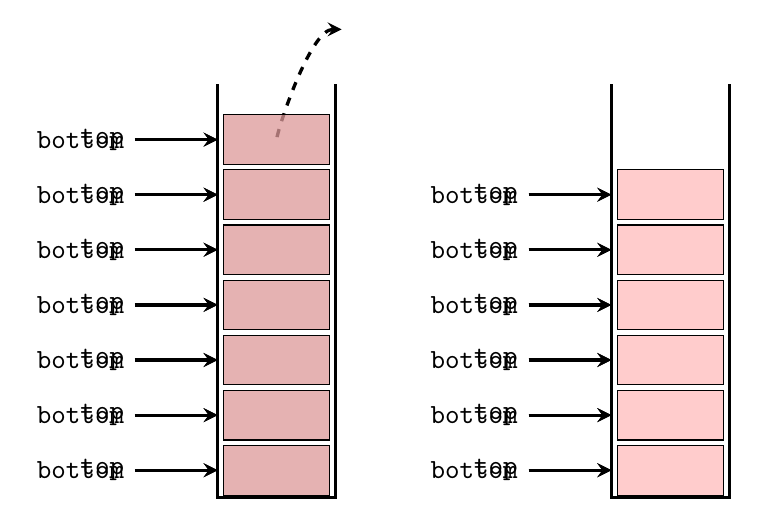
\begin{tikzpicture}
    \tikzstyle{information text}=[rounded corners,fill=blue!20,inner sep=1ex]

    \def\x{1.5}
    \def\y{0.7}
    \def\r{0.5}
    \def\c{9}
    
    \draw[<-,>=stealth,dashed,very thick] (\r+2.05*\x,\c*\y-0.5*\y) .. controls +(left:4mm) and +(up:1mm) .. (2+0.5*\x,6.5*\y);

    \def\r{2}
    \draw[very thick] (\r,7.5*\y)--(\r,0*\y)--(\r+\x,0*\y)--(\r+\x,7.5*\y);
    \foreach \c in {1,2,...,7}{
      \ifthenelse{\c=7}{
        \filldraw[fill=black!40,fill opacity=0.5] (\r+0.05*\x,\c*\y-0.95*\y)rectangle(\r+0.95*\x,\c*\y-0.05*\y);
        \draw[->,>=stealth,very thick] (\r-0.7*\x,\c*\y-0.5*\y) node[left] {\tt{top}}--(\r+0,\c*\y-0.5*\y);
      }{
        \filldraw[fill=red!40,fill opacity=0.5] (\r+0.05*\x,\c*\y-0.95*\y)rectangle(\r+0.95*\x,\c*\y-0.05*\y);
      }
      
      \ifthenelse{\c=1}{
        \draw[->,>=stealth,very thick] (\r-0.7*\x,\c*\y-0.5*\y) node[left] {\tt{bottom}}--(\r+0,\c*\y-0.5*\y);
      }{}
      
    }

    \pause 

    \def\r{7}
    \draw[very thick] (\r,7.5*\y)--(\r,0*\y)--(\r+\x,0*\y)--(\r+\x,7.5*\y);
    \foreach \c in {1,2,...,6}{
      \filldraw[fill=red!40,fill opacity=0.5] (\r+0.05*\x,\c*\y-0.95*\y)rectangle(\r+0.95*\x,\c*\y-0.05*\y);
      \ifthenelse{\c=1}{
        \draw[->,>=stealth,very thick] (\r-0.7*\x,\c*\y-0.5*\y) node[left] {\tt{bottom}}--(\r+0,\c*\y-0.5*\y);
      }{}
      \ifthenelse{\c=6}{
        \draw[->,>=stealth,very thick] (\r-0.7*\x,\c*\y-0.5*\y) node[left] {\tt{top}}--(\r+0,\c*\y-0.5*\y);
      }{}
    }
  \end{tikzpicture}
  \caption{出栈}
\end{figure}


\end{frame}


\begin{frame}[fragile]\ft{\subsecname}   
\begin{lstlisting}[mathescape=true]
    ADT Stack{
      Data:
      `同线性表。元素具有相同的数据类型,相邻元素有前驱、后继关系。`
      Operation:
      Init(*S):     `初始化操作,创建一个空栈S`
      Destroy(*S):  `若栈存在,销毁之`
      Clear(*S):    `将栈清空`
      IsEmpty(S):   `若栈为空,返回true;否则返回false`
      GetTop(S,*e): `若栈存在且非空,用e返回栈顶元素`
      Push(*S,e):   `若栈存在,插入新元素e并称为栈顶元素`
      Pop(*S,*e):   `删除栈顶元素,并用e返回其值`
      Length(S):   `返回元素个数`
    } ADT Stack
  \end{lstlisting}
\end{frame}

\subsection{顺序栈}

% \begin{frame}\ft{\subsecname}
%   既然栈是线性表的特例,那么栈的顺序存储其实是线性表顺序存储的简化。
%   栈的顺序存储结构简称顺序栈,。根据数组是否可以根据需要增大,又可分为静态顺序栈和动态顺序栈。
% \begin{itemize}
% \item[$\diamond$]
% 静态顺序栈实现简单,但不能根据需要增大栈的存储空间;
% \item[$\diamond$]
% 动态顺序栈可以根据需要增大栈的存储空间,但实现稍微复杂。
% \end{itemize}

% \end{frame}

\begin{frame}\ft{\subsecname}
  既然栈是线性表的特例,那么栈的顺序存储其实是线性表顺序存储的简化。
  栈的顺序存储结构简称顺序栈,用数组来实现。 \vskip.1in

  \pause
  \begin{wenti}
    对于栈,用数组哪一端作为栈顶或栈底会比较好?
  \end{wenti} \vskip.1in

  \pause
  下标为0的一端作为栈底比较好,因为首元素都存在栈底,变化最小。
\end{frame}
%
%
\begin{frame}[fragile]\ft{\subsecname}
  \begin{lstlisting}[title=栈的结构定义,language=C]
    #define MAXSIZE 100
    typedef int ElemType;
    typedef struct SqStack{
      ElemType data[MAXSIZE];
      int top;
    }SqStack;
  \end{lstlisting}

  \begin{itemize}
  \item {\tt top}用于指示栈顶元素在数组中的位置,它必须小于存储栈的长度{\tt StackSize};
  \item 当栈存在一个元素时,{\tt top == 0},因此通常把空栈的判定条件定为{\tt top == -1}.
  \end{itemize}
\end{frame}
%
%
\begin{frame}\ft{\subsecname}
  \begin{figure}
  \centering
  \begin{tikzpicture}
    \tikzstyle{information text}=[fill=white,inner sep=1ex]
    \def\x{1.5}
    \def\y{0.7}


    \def\r{0}    
    \draw[very thick] (\r,5*\y)--(\r,0*\y)--(\r+\x,0*\y)--(\r+\x,5*\y);
    \node[below,style=information text]at(\r+0.5*\x,-1*\y){有两个元素,{\tt top=1}};
    \foreach \c in {1,2,...,5}{
      \edef\cc{\number\numexpr\c-1\relax}
      \node[left] at (\r+0*\x,\c*\y-0.5*\y) {\cc};
      \ifthenelse{\c=1 \OR \c=2}{
        \node [] at (\r+0.5*\x,\c*\y-0.5*\y) {$a_\c$};
        \filldraw[fill=red!40,fill opacity=0.5] (\r+0.05*\x,\c*\y-0.95*\y)rectangle(\r+0.95*\x,\c*\y-0.05*\y);
        \ifthenelse{\c=2}{          
          \draw[->,>=stealth,very thick] (\r-\x,\c*\y-0.5*\y) --node[above] {{\tt top}}(\r-0.4*\x,\c*\y-0.5*\y);
        }{}
      }{
        \filldraw[fill=white,fill opacity=0.5] (\r+0.05*\x,\c*\y-0.95*\y)rectangle(\r+0.95*\x,\c*\y-0.05*\y);     }
    }

    \pause 
    %% 
    \def\r{4}    
    \draw[very thick] (\r,5*\y)--(\r,0*\y)--(\r+\x,0*\y)--(\r+\x,5*\y);
    \node[below,style=information text]at(\r+0.5*\x,-1*\y){空栈,{\tt top=-1}};
    \foreach \c in {1,2,...,5}{
      \edef\cc{\number\numexpr\c-1\relax}
      \node[left] at (\r+0*\x,\c*\y-0.5*\y) {\cc};
      \filldraw[fill=white,fill opacity=0.5] (\r+0.05*\x,\c*\y-0.95*\y)rectangle(\r+0.95*\x,\c*\y-0.05*\y); 
    }
    \def\c{0}
    \draw[->,>=stealth,very thick] (\r-\x,\c*\y-0.5*\y) --node[above] {{\tt top}}(\r-0.4*\x,\c*\y-0.5*\y);


    \pause 
    %% 
    \def\r{8}    
    \draw[very thick] (\r,5*\y)--(\r,0*\y)--(\r+\x,0*\y)--(\r+\x,5*\y);
    \node[below,style=information text]at(\r+0.5*\x,-1*\y){栈满,{\tt top=4}};
    \foreach \c in {1,2,...,5}{
      \edef\cc{\number\numexpr\c-1\relax}
      \node[left] at (\r+0*\x,\c*\y-0.5*\y) {\cc};
      \node [] at (\r+0.5*\x,\c*\y-0.5*\y) {$a_\c$};
      \filldraw[fill=red!40,fill opacity=0.5] (\r+0.05*\x,\c*\y-0.95*\y)rectangle(\r+0.95*\x,\c*\y-0.05*\y);
    }
    \def\c{5}
    \draw[->,>=stealth,very thick] (\r-\x,\c*\y-0.5*\y) --node[above] {{\tt top}}(\r-0.4*\x,\c*\y-0.5*\y);



  \end{tikzpicture}
\end{figure}

\end{frame}
%
\begin{frame}\ft{\subsecname}
  \begin{figure}
  \centering
  \begin{tikzpicture}
    \tikzstyle{information text}=[fill=white,inner sep=1ex]
    \def\x{1.5}
    \def\y{0.7}


    \def\r{0}    
    \draw[very thick] (\r,5*\y)--(\r,0*\y)--(\r+\x,0*\y)--(\r+\x,5*\y);
    \node[below,style=information text]at(\r+0.5*\x,-1*\y){数组{\tt data}};
    \foreach \c in {1,2,...,5}{
      \edef\cc{\number\numexpr\c-1\relax}
      \node[left] at (\r+0*\x,\c*\y-0.5*\y) {\cc};
      \ifthenelse{\c=1 \OR \c=2}{
        \node [] at (\r+0.5*\x,\c*\y-0.5*\y) {$a_\c$};
        \filldraw[fill=red!40,fill opacity=0.5] (\r+0.05*\x,\c*\y-0.95*\y)rectangle(\r+0.95*\x,\c*\y-0.05*\y);
        \ifthenelse{\c=2}{          
          \draw[->,>=stealth,very thick] (\r-\x,\c*\y-0.5*\y) --node[above] {{\tt top}}(\r-0.4*\x,\c*\y-0.5*\y);
        }{}
      }{
        \filldraw[fill=white,fill opacity=0.5] (\r+0.05*\x,\c*\y-0.95*\y)rectangle(\r+0.95*\x,\c*\y-0.05*\y);     }
    }

    \pause 
    %% 
    \def\r{4}    
    \draw[very thick] (\r,5*\y)--(\r,0*\y)--(\r+\x,0*\y)--(\r+\x,5*\y);
    \node[below,style=information text]at(\r+0.5*\x,-1*\y){元素{\tt e}进栈};
    \foreach \c in {1,2,...,5}{
      \edef\cc{\number\numexpr\c-1\relax}
      \node[left] at (\r+0*\x,\c*\y-0.5*\y) {\cc};
      \ifthenelse{\c=1 \OR \c=2 \OR \c=3}{
        \ifthenelse{\c=3}{
          \node [] at (\r+0.5*\x,\c*\y-0.5*\y) {$e$};
          \filldraw[fill=blue!40,fill opacity=0.5] (\r+0.05*\x,\c*\y-0.95*\y)rectangle(\r+0.95*\x,\c*\y-0.05*\y);
          \draw[->,>=stealth,very thick] (\r-\x,\c*\y-0.5*\y) --node[above] {{\tt top}}(\r-0.4*\x,\c*\y-0.5*\y);
        }{
          \node [] at (\r+0.5*\x,\c*\y-0.5*\y) {$a_\c$};
          \filldraw[fill=red!40,fill opacity=0.5] (\r+0.05*\x,\c*\y-0.95*\y)rectangle(\r+0.95*\x,\c*\y-0.05*\y);
        }
      }{
        \filldraw[fill=white,fill opacity=0.5] (\r+0.05*\x,\c*\y-0.95*\y)rectangle(\r+0.95*\x,\c*\y-0.05*\y);     }
    }


  \end{tikzpicture}
\end{figure}

\end{frame}
%
\begin{frame}[fragile]\ft{\subsecname}
  \lstinputlisting[
    title={\tt Push.c},
    language=C,
  ]{Chapters/Ch03/Code/SqStack/Push.c}
\end{frame}

\begin{frame}\ft{\subsecname}
  \begin{figure}
\centering
\begin{tikzpicture}
\tikzstyle{information text}=[fill=white,inner sep=1ex]
\def\x{1.5}
\def\y{0.7}



%% 
\def\r{0}    
\draw[very thick] (\r,5*\y)--(\r,0*\y)--(\r+\x,0*\y)--(\r+\x,5*\y);
\node[below,style=information text]at(\r+0.5*\x,-1*\y){数组{\tt data}};
\foreach \c in {1,2,...,5}{
\edef\cc{\number\numexpr\c-1\relax}
\node[left] at (\r+0*\x,\c*\y-0.5*\y) {\cc};
\ifthenelse{\c=1 \OR \c=2 \OR \c=3}{
\ifthenelse{\c=3}{
  \node [] at (\r+0.5*\x,\c*\y-0.5*\y) {$e$};
  \filldraw[fill=blue!40,fill opacity=0.5] (\r+0.05*\x,\c*\y-0.95*\y)rectangle(\r+0.95*\x,\c*\y-0.05*\y);
  \draw[->,>=stealth,very thick] (\r-\x,\c*\y-0.5*\y) --node[above] {{\tt top}}(\r-0.4*\x,\c*\y-0.5*\y);
}{
  \node [] at (\r+0.5*\x,\c*\y-0.5*\y) {$a_\c$};
  \filldraw[fill=red!40,fill opacity=0.5] (\r+0.05*\x,\c*\y-0.95*\y)rectangle(\r+0.95*\x,\c*\y-0.05*\y);
}
}{
\filldraw[fill=white,fill opacity=0.5] (\r+0.05*\x,\c*\y-0.95*\y)rectangle(\r+0.95*\x,\c*\y-0.05*\y);     }
}

\pause
\def\r{4}    
\draw[very thick] (\r,5*\y)--(\r,0*\y)--(\r+\x,0*\y)--(\r+\x,5*\y);
\node[below,style=information text]at(\r+0.5*\x,-1*\y){元素{\tt e}出栈};
\foreach \c in {1,2,...,5}{
\edef\cc{\number\numexpr\c-1\relax}
\node[left] at (\r+0*\x,\c*\y-0.5*\y) {\cc};
\ifthenelse{\c=1 \OR \c=2}{
\node [] at (\r+0.5*\x,\c*\y-0.5*\y) {$a_\c$};
\filldraw[fill=red!40,fill opacity=0.5] (\r+0.05*\x,\c*\y-0.95*\y)rectangle(\r+0.95*\x,\c*\y-0.05*\y);
\ifthenelse{\c=2}{          
  \draw[->,>=stealth,very thick] (\r-\x,\c*\y-0.5*\y) --node[above] {{\tt top}}(\r-0.4*\x,\c*\y-0.5*\y);
}{}
}{
\filldraw[fill=white,fill opacity=0.5] (\r+0.05*\x,\c*\y-0.95*\y)rectangle(\r+0.95*\x,\c*\y-0.05*\y);     }
}



\end{tikzpicture}
\end{figure}

\end{frame}

\begin{frame}[fragile]\ft{\subsecname}
  \lstinputlisting[
    title={\tt Pop.c},
    language=C,
  ]{Chapters/Ch03/Code/SqStack/Pop.c}
\end{frame}


\begin{frame}[fragile]
\begin{center}
  \textcolor{acolor5}{\Large 顺序栈之完整程序}
\end{center}
\end{frame}
\begin{frame}[fragile,allowframebreaks]\ft{\tt SqStack.h}
  \lstinputlisting[
    language=C,
  ]{Chapters/Ch03/Code/SqStack/SqStack.h}
\end{frame}

\begin{frame}[fragile]\ft{\tt Init.c}
  \lstinputlisting[
    language=C,
  ]{Chapters/Ch03/Code/SqStack/Init.c}
\end{frame}

\begin{frame}[fragile]\ft{\tt PrintS.c}
  \lstinputlisting[
    language=C,
  ]{Chapters/Ch03/Code/SqStack/PrintS.c}
\end{frame}

\begin{frame}[fragile]\ft{\tt Push.c}
  \lstinputlisting[
    language=C,
  ]{Chapters/Ch03/Code/SqStack/Push.c}
\end{frame}

\begin{frame}[fragile]\ft{\tt Pop.c}
  \lstinputlisting[
    language=C,
  ]{Chapters/Ch03/Code/SqStack/Pop.c}
\end{frame}

\begin{frame}[fragile]\ft{\tt Clear.c}
  \lstinputlisting[
    language=C,
  ]{Chapters/Ch03/Code/SqStack/Clear.c}
\end{frame}

\begin{frame}[fragile]\ft{\tt Destroy.c}
  \lstinputlisting[
    language=C,
  ]{Chapters/Ch03/Code/SqStack/Destroy.c}
\end{frame}


\subsection{两栈共享空间}

\begin{frame}\ft{\subsecname}
\begin{wenti}
设有两个相同类型的栈,为它们各自开辟数组空间,极有可能第一个栈满,而另一个栈还有很多空闲空间。
请问如何更有效地利用存储空间?
\end{wenti}
\pause
可以用一个数组来存储两个栈,实现两栈共享空间。
\end{frame}
%
%
\begin{frame}\ft{\subsecname}
\begin{figure}
  \centering
  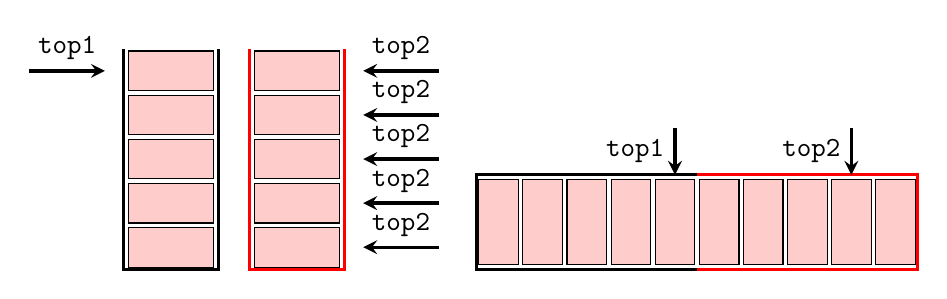
\begin{tikzpicture}[scale=0.8]
    \tikzstyle{information text}=[fill=white,inner sep=1ex]
    \def\x{1.5}
    \def\y{0.7}

    %% 
    \def\r{0}    
    \draw[very thick] (\r,5*\y)--(\r,0*\y)--(\r+\x,0*\y)--(\r+\x,5*\y);
    \foreach \c in {1,2,...,5}{
      \edef\cc{\number\numexpr\c-1\relax}
      \filldraw[fill=red!40,fill opacity=0.5] (\r+0.05*\x,\c*\y-0.95*\y)rectangle(\r+0.95*\x,\c*\y-0.05*\y);
    }
    \def\c{5}
    \draw[->,>=stealth,very thick] (\r-\x,\c*\y-0.5*\y) --node[above] {{\tt top1}}(\r-0.2*\x,\c*\y-0.5*\y);

    \def\r{2}    
    \draw[red,very thick] (\r,5*\y)--(\r,0*\y)--(\r+\x,0*\y)--(\r+\x,5*\y);
    \foreach \c in {1,2,...,5}{
      \ifthenelse{\c=1 \OR \c=2}{
        \filldraw[fill=red!40,fill opacity=0.5] (\r+0.05*\x,\c*\y-0.95*\y)rectangle(\r+0.95*\x,\c*\y-0.05*\y);
        \ifthenelse{\c=2}{          
          \draw[->,>=stealth,very thick] (\r+2*\x,\c*\y-0.5*\y) --node[above] {{\tt top2}}(\r+1.2*\x,\c*\y-0.5*\y);
        }{}
      }{
        %% \filldraw[fill=white,fill opacity=0.5] (\r+0.05*\x,\c*\y-0.95*\y)rectangle(\r+0.95*\x,\c*\y-0.05*\y);
      }
    }

    \pause 
    %% 
    \def\c{0}
    \def\r{8}
    \draw[very thick] (\r*\y+5*\y,0*\x)--(\r*\y+0*\y,0*\x)--(\r*\y+0*\y,1*\x)--(\r*\y+5*\y,1*\x);
    \foreach \r in {8,...,12}{
      \filldraw[fill=red!40,fill opacity=0.5] (\r*\y+0.05*\y,0.05*\x)rectangle(\r*\y+0.95*\y,0.95*\x);
    }
    \def\c{5}
    \draw[->,>=stealth,very thick] (12.5*\y,1.5*\x) --node[left] {{\tt top1}}(12.5*\y,1.*\x);

    %% 
    \def\c{0}
    \def\r{13}
    \draw[red,very thick] (\r*\y+0*\y,0*\x)--(\r*\y+5*\y,0*\x)--(\r*\y+5*\y,1*\x)--(\r*\y+0*\y,1*\x);
    \foreach \r in {13,...,17}{
      \ifthenelse{\r=16 \OR \r=17 }{
        \filldraw[fill=red!40,fill opacity=0.5] (\r*\y+0.05*\y,0.05*\x)rectangle(\r*\y+0.95*\y,0.95*\x);
      }{}
    }
    \def\c{5}
    \draw[->,>=stealth,very thick] (16.5*\y,1.5*\x) --node[left] {{\tt top2}}(16.5*\y,1.*\x);


  \end{tikzpicture}
\end{figure}

\end{frame}
%
%
\begin{frame}\ft{\subsecname}
\begin{itemize}
\item   让一个栈的栈底为数组的始端,另一个栈的栈底为数组的末端。
这样,两个栈如果增加元素,就是两端点向中间延伸。 \\
\item 设{\tt top1}和{\tt top2}分别是栈1和栈2的栈顶指针,只要它们俩不碰面,两个栈就可以一直使用。
\end{itemize}
\end{frame}
%
%
\begin{frame}\ft{\subsecname}
栈满的情形:
\begin{itemize}
\item 栈1为空({\tt top1 == -1}),栈1为满({\tt top2 == 0})
\item 栈2为空({\tt top2 == n}),栈1为满({\tt top1 == n-1})
\item 一般情形: 两个栈见面即栈满,亦即{\tt top1+1 == top2}。
\end{itemize}
\end{frame}
%
%
\begin{frame}[fragile]\ft{\subsecname:{\tt Share\_SqStack.h}}
\lstinputlisting[
language=C,
]{Chapters/Ch03/Code/ShareSqStack/Share_SqStack.h}

\end{frame}

\begin{frame}[fragile]\ft{\subsecname:{\tt Push.c}}
\lstinputlisting[
language=C,
]{Chapters/Ch03/Code/ShareSqStack/Push.c}

\end{frame}


\begin{frame}[fragile]\ft{\subsecname:{\tt Pop.c}}
\lstinputlisting[
language=C,
]{Chapters/Ch03/Code/ShareSqStack/Pop.c}

\end{frame}
%
%

\subsection{链栈}
\begin{frame}[fragile]\ft{\subsecname}
\begin{dingyi}
栈的链式存储结构称为链栈,是操作受限的单链表,其插入和删除操作只能在表头位置上进行。
\end{dingyi}
\end{frame}

\begin{frame}[fragile]\ft{\subsecname}
\begin{figure}
\centering
\begin{tikzpicture}
\tikzstyle{information text}=[rounded corners,fill=blue!10,inner sep=1ex]
\def\x{1}
\def\y{0.6}

\foreach \r in {0,4}{
\ifthenelse{\r=4}{
\foreach \c in {6,4,2,0}{
\draw[thick,fill=red!10,rounded corners](\r*\x,\c*\y)rectangle(\r*\x+1.5*\x,\c*\y+\y);
\draw[thick] (\r*\x+\x,\c*\y)--(\r*\x+\x,\c*\y+\y);
\ifthenelse{6=\c}{\node[]at(\r*\x+0.5*\x,\c*\y+0.5*\y){$a_4$};}{}
\ifthenelse{4=\c}{\node[]at(\r*\x+0.5*\x,\c*\y+0.5*\y){$a_3$};}{}
\ifthenelse{2=\c}{\node[]at(\r*\x+0.5*\x,\c*\y+0.5*\y){$a_2$};}{}
\ifthenelse{0=\c}{
\node[]at(\r*\x+0.5*\x,\c*\y+0.5*\y){$a_1$};            
}{}

\ifthenelse{6=\c}{
\draw[->,thick] (\r*\x-0.6*\x,\c*\y+0.5*\y)node[left]{{\tt top}} --(\r*\x-0.1*\x,\c*\y+0.5*\y);
}{}

\draw[->,thick] (\r*\x+1.25*\x,\c*\y+0.5*\y) --(\r*\x+1.25*\x,\c*\y-0.9*\y);

\ifthenelse{\c=0} {
\filldraw[thick] (\r*\x+\x,\c*\y-1.5*\y) rectangle (\r*\x+1.5*\x,\c*\y-\y);
\node[below] at (\r*\x+0.75*\x,\c*\y-2*\y) {非空栈};
}

}
}
%{\foreach \c in {6}{
%\draw[thick,fill=red!10,rounded corners](\r*\x,\c*\y)rectangle(\r*\x+1.5*\x,\c*\y+\y);
%\draw[thick] (\r*\x+\x,\c*\y)--(\r*\x+\x,\c*\y+\y);
%\draw[->,>=stealth] (\r*\x-0.5*\x,\c*\y+0.5*\y)node[left]{{\tt top}} --(\r*\x,\c*\y+0.5*\y);
%
%\draw[->,thick] (\r*\x+1.25*\x,\c*\y+0.5*\y) --(\r*\x+1.25*\x,\c*\y-0.9*\y);
%\filldraw[thick] (\r*\x+\x,\c*\y-1.5*\y) rectangle (\r*\x+1.5*\x,\c*\y-\y);
%\node[below] at (\r*\x+0.75*\x,\c*\y-2*\y) {空栈};
%}
%}
}
\end{tikzpicture}
\end{figure}

\end{frame}
%
%
\begin{frame}[fragile]\ft{\subsecname}
\begin{itemize}
\item 对于链栈,通常不需要头结点;\\[0.1in]
\item 对于链栈,基本不存在栈满的情况;\\[0.1in]
\item 对于空栈,通常指的是{\tt top == NULL}.
\end{itemize}
\end{frame}
%




\begin{frame}
\begin{center}
\textcolor{acolor5}{\Large 链栈之完整程序}
\end{center}
\end{frame}
%




\begin{frame}[fragile,allowframebreaks]\ft{{\tt linkstack.h}}
\lstinputlisting[
language=C,
]{Chapters/Ch03/Code/LinkStack/LinkStack.h}
\end{frame}



\begin{frame}[fragile]\ft{{\tt Init.c}}
\lstinputlisting[
language=C,
]{Chapters/Ch03/Code/LinkStack/Init.c}
\end{frame}
%
\begin{frame}[fragile]\ft{{\tt Push.c}}
\lstinputlisting[
language=C,
]{Chapters/Ch03/Code/LinkStack/Push.c}
\end{frame}
%
\begin{frame}[fragile]\ft{{\tt Pop.c}}
\lstinputlisting[
language=C,
]{Chapters/Ch03/Code/LinkStack/Pop.c}
\end{frame}
%
\begin{frame}[fragile]\ft{{\tt PrintS.c}}
\lstinputlisting[
language=C,
]{Chapters/Ch03/Code/LinkStack/PrintS.c}
\end{frame}
%
\begin{frame}[fragile]\ft{{\tt main.c}}
\lstinputlisting[
language=C,
]{Chapters/Ch03/Code/LinkStack/main.c}
\end{frame}

\subsection{栈的应用}

\begin{frame}\ft{\subsecname}
由于栈“后进先出”的固有特性,故栈是程序设计中常用的工具和数据结构。
\end{frame}

\begin{frame}\ft{应用1:数制转换}
十进制整数$n$向其它进制数$d(=2, 8, 16)$的转换是计算机实现计算的基本问题。

\textcolor{acolor5}{转换法则:}
$$
n=(n\div d)\times d+ r
$$
其中$r$为余数,且$0\le r < d$。
\end{frame}

\begin{frame}\ft{应用1:数制转换}
\begin{li}
$(1348)_{10}=(2504)_8$,其运算过程如下:
\begin{table}
\begin{tabular}{ccc}\hline
$n$ & $n\div 8$ & $r$\\ \hline
1348 & 168 & 4\\
168  & 21  & 0\\
21   & 2   & 5\\
2    & 0   & 2\\\hline
\end{tabular}
\end{table}
\end{li}
\end{frame}
%
\begin{frame}[fragile,allowframebreaks]\ft{应用1:数制转换(程序)}
\lstinputlisting[
language=c,
]{Chapters/Ch03/Code/App/App1/Convert.c}
\end{frame}
%

\begin{frame}\ft{应用2:括号匹配}
在文字处理软件或编写程序时,常常需要检查一个字符串或一个表达式终端括号是否相匹配?
\vspace{0.1in}

\pause 
\textcolor{acolor5}{匹配思想:}
从左至右扫描一个字符串(或表达式),则\textcolor{acolor1}{每个右括号将于最近遇到的那个左括号相匹配}。可以在从左到右扫描过程中把所遇到的左括号存放到堆栈中,每当遇到一个右括号时,就将它与栈顶的左括号(如果存在)相匹配,同时从栈顶删除该左括号。  

\end{frame}


\begin{frame}\ft{应用2:括号匹配}
\textcolor{acolor5}{算法思想:}
设置一个栈,当读到左括号时,左括号进栈。当读到右括号时,则从栈中弹出一个元素,与读到的左括号进行匹配,若匹配成功,继续读入;否则匹配失败,返回{\tt FALSE}.    


\end{frame}

\begin{frame}[fragile,allowframebreaks]\ft{应用2:括号匹配(程序)}
\lstinputlisting[
language=C,
]{Chapters/Ch03/Code/App/App2/MatchBrackets.c}
\end{frame}

\begin{frame}\ft{前缀、中缀、后缀表达式}
它们都是对表达式的记法,其区别在于运算符相对操作数的位置不同:
\begin{itemize}
\item 前缀表达式:运算符位于其相关操作数的前面;
\item 中缀表达式:运算符位于其相关操作数的中间;
\item 后缀表达式:运算符位于其相关操作数的后面。
\end{itemize}
\end{frame}

\begin{frame}\ft{前缀、中缀、后缀表达式}
例如:
\begin{itemize}
\item 前缀表达式:$-~\times~+~3~4~5~6$
\item 中缀表达式:$(3~+~4)~\times ~5 ~- ~6$
\item 后缀表达式:$3~4~+~5~\times~6~-$
\end{itemize}
\end{frame}

\begin{frame}\ft{前缀、中缀、后缀表达式}
\textcolor{acolor3}{中缀表达式:}
人们常用的算术表示方法。

中缀表达式很容易被人的大脑理解和分析,但对计算机来说却是很复杂的。因此计算表达式的值时,通常需要将中缀表达式转换为前缀或后缀表达式,然后进行求值。

\textcolor{acolor5}{对计算机来说,计算前缀或后缀表达式的值非常简单。}
\end{frame}

\begin{frame}\ft{前缀、中缀、后缀表达式}
\textcolor{acolor3}{前缀表达式:} 也称“前缀记法、波兰式”,其运算符位于操作数之前。\vspace{0.1in}

\textcolor{acolor3}{后缀表达式:} 也称“后缀记法、逆波兰式”,其运算符位于操作数之后。
\end{frame}

\begin{frame}\ft{应用3:后缀表达式的计算机求值}
从左到右扫描表达式,
\begin{itemize}
\item[(1)] 遇到操作数,将数字入栈;
\item[(2)] 遇到运算符,弹出栈顶的两个数;
\item[(3)] 将这两个数用运算符做相应计算(次顶元素~op~栈顶元素),并将结果入栈;
\item[(4)] 重复(1)-(3)直到表达式右端,最后运算出的值即为表达式的结果。
\end{itemize}
\end{frame}

\begin{frame}\ft{应用3:后缀表达式的计算机求值}
\begin{li}
以后缀表达式
$$
3~4~+~5~\times~6~-
$$
为例,详解整个过程。
\end{li}
\end{frame}

\begin{frame}\ft{应用3:后缀表达式的计算机求值}
\begin{enumerate}
\item 将{\tt 3}和{\tt 4}入栈;
\item 遇到{\tt +},弹出{\tt 4}和{\tt 3},计算{\tt 3+4=7},再将{\tt 7}入栈;
\item 将{\tt 5}入栈;
\item 遇到{\tt *},弹出{\tt 5}和{\tt 7},计算{\tt 7*5=3},再将{\tt 35}入栈;
\item 将{\tt 6}入栈;
\item 遇到{\tt -},弹出{\tt 6}和{\tt 35},计算{\tt 35-6=29},即为最终结果。
\end{enumerate}
\end{frame}

\begin{frame}\ft{应用4:将中缀表达式转换为后缀表达式}
\begin{itemize}
\item[1] 初始化两个栈:运算符栈{\tt S1}和存储中间结果的栈{\tt S2};\\[0.1in]
\item[2] 从左到右扫描中缀表达式;\\[0.1in]
\item[3] 遇到操作数时,将其压入{\tt S2};
\end{itemize}
\end{frame}

\begin{frame}\ft{应用4:将中缀表达式转换为后缀表达式}
\begin{itemize}
\item[4] 遇到运算符,比较其与{\tt S1}栈顶运算符的优先级:\\[0.1in]
\begin{itemize}
\item[4.1] 若{\tt S1}为空,或栈顶运算符为“(”,则压入{\tt S1};\\[0.1in]
\item[4.2] 否则,若其优先级高于栈顶运算符,则压入{\tt S1};\\[0.1in]
\item[4.3] 否则,将{\tt S1}的栈顶运算符弹出并压入到{\tt S2}中,再次转到4.1与{\tt S1}中新的栈顶运算符做比较;
\end{itemize}
\end{itemize}
\end{frame}

\begin{frame}\ft{应用4:将中缀表达式转换为后缀表达式}
\begin{itemize}
\item[5] 遇到括号时,\\[0.1in]
\begin{itemize}
\item[5.1] 如果是“(”,则压入{\tt S1};\\[0.1in]
\item[5.2] 如果是“)”,则依次弹出{\tt S1}的栈顶元素,并压入S2,直到遇到“(”为止,此时这一对括号丢弃;
\end{itemize}
\end{itemize}
\end{frame}

\begin{frame}\ft{应用4:将中缀表达式转换为后缀表达式}
\begin{itemize}
\item[6] 重复步骤2-5,直到表达式的最右端;\\[0.1in]
\item[7] 将{\tt S1}中剩余的运算符依次弹出并压入S2;\\[0.1in]
\item[8] 依次弹出{\tt S2}中的元素并输出,结果的逆序即为对应的后缀表达式。
\end{itemize}
\end{frame}



\begin{frame}\ft{应用4:将中缀表达式转换为后缀表达式}
\begin{scriptsize}
\begin{table}
\centering
\caption{{\tt 中缀表达式 1 + ((2 + 3) + 4) * 5}}
\begin{tabular}{|c|l|l|}\hline
{\tt 扫描到的字符} & {\tt S2(栈底->栈顶)} & {\tt S1(栈底->栈顶)} \\\hline
{\tt 1} &   {\tt 1} &         \\\hline 
{\tt +} &   {\tt 1} &  {\tt +}\\\hline 
{\tt (} &   {\tt 1} &  {\tt +(}\\\hline 
{\tt (} &   {\tt 1} &  {\tt +((}\\\hline 
{\tt 2} &   {\tt 12} &  {\tt +((}\\\hline 
{\tt +} &   {\tt 12} &  {\tt +((+}\\\hline 
{\tt 3} &   {\tt 123} &  {\tt +((+}\\\hline 
{\tt )} &   {\tt 123+} &  {\tt +(}\\\hline 
{\tt +} &   {\tt 123+} &  {\tt +(+}\\\hline 
{\tt 4} &   {\tt 123+4} &  {\tt +(+}\\\hline 
{\tt )} &   {\tt 123+4+} &  {\tt +}\\\hline 
{\tt *} &   {\tt 123+4} &  {\tt +*}\\\hline 
{\tt 5} &   {\tt 123+45} &  {\tt +*}\\\hline 
        &   {\tt 123+45*+} &  \\\hline 
\end{tabular}
\end{table}
\end{scriptsize}
\end{frame}


\begin{frame}\ft{应用4:将中缀表达式转换为后缀表达式}
\begin{scriptsize}
\begin{table}
\centering
\caption{{\tt 中缀表达式 1 + ((2 + 3) * 4) - 5}}
\begin{tabular}{|c|l|l|}\hline
{\tt 扫描到的字符} & {\tt S2(栈底->栈顶)} & {\tt S1(栈底->栈顶)} \\\hline
{\tt 1} &   {\tt 1} &         \\\hline 
{\tt +} &   {\tt 1} &  {\tt +}\\\hline 
{\tt (} &   {\tt 1} &  {\tt +(}\\\hline 
{\tt (} &   {\tt 1} &  {\tt +((}\\\hline 
{\tt 2} &   {\tt 12} &  {\tt +((}\\\hline 
{\tt +} &   {\tt 12} &  {\tt +((+}\\\hline 
{\tt 3} &   {\tt 123} &  {\tt +((+}\\\hline 
{\tt )} &   {\tt 123+} &  {\tt +(}\\\hline 
{\tt *} &   {\tt 123+} &  {\tt +(*}\\\hline 
{\tt 4} &   {\tt 123+4} &  {\tt +(+}\\\hline 
{\tt )} &   {\tt 123+4*} &  {\tt +}\\\hline 
{\tt -} &   {\tt 123+4+} &  {\tt -}\\\hline 
{\tt 5} &   {\tt 123+4+5} &  {\tt -}\\\hline 
        &   {\tt 123+4+5-} &  \\\hline 
\end{tabular}
\end{table}
\end{scriptsize}
\end{frame}











%% \subsubsection{栈的动态顺序存储表示}
%% \begin{frame}\ft{\subsecname}
%% 采用动态一维数组来存储栈。所谓动态,指的是栈的大小可以根据需要增加。
%% \begin{itemize}
%% \item[$\diamond$]
%% 用$bottom$表示栈底指针,栈底固定不变;
%% \item[]
%% 栈顶随着进栈和退栈操作而变化,用栈顶指针$top$指示当前栈顶位置。
%% \item[$\diamond$]
%% 用$top=bottom$作为栈空的标记,每次$top$指向栈顶数组中的下一个存储位置。
%% \item[$\diamond$] \red{结点进栈}:首先将数据元素保存到栈顶,然后执行$top$加1,使$top$指向栈顶的下一个存储位置。
%% \item[$\diamond$] \red{结点出栈}:首先执行$top$减1,使$top$指向栈顶元素的存储位置,然后将栈顶元素取出。
%% \end{itemize}
%% \end{frame}


%% \begin{frame}\ft{\subsecname}
%% \begin{figure}
%% \centering
%% \begin{tikzpicture}
%%   \tikzstyle{information text}=[rounded corners,fill=blue!10,inner sep=1ex]
%% \def\x{1}
%% \def\y{0.5}

%% \def\r{8}
%% \foreach \r in {0,4,8}{
%% \foreach \c in {1,2,...,5}{
%% \filldraw[fill=red!20,fill opacity=0.5] (\r+0,\c*\y-\y)rectangle(\r+\x,\c*\y);

%% \ifthenelse{0=\r \AND 1=\c}
%% {\draw[->,>=stealth] (\r-0.5,\c*\y-0.8*\y)node[left]{$bottom$}--(\r,\c*\y-0.8*\y);
%% \draw[->,>=stealth] (\r-0.5,\c*\y-0.2*\y)node[left]{$top$}--(\r,\c*\y-0.2*\y);
%% \node[below] at (\r+0.5*\x,\c*\y-\y){空栈};
%% }
%% {}

%% \ifthenelse{4=\r \AND 1=\c}
%% {\draw[->,>=stealth] (\r-0.5,\c*\y-0.5*\y)node[left]{$bottom$}--(\r,\c*\y-0.5*\y);
%% \node[] at (\r+0.5*\x,\c*\y-0.5*\y){$a$};
%% \node[below] at (\r+0.5*\x,\c*\y-\y){元素$a$进栈};
%% }{}

%% \ifthenelse{4=\r \AND 2=\c}
%% {\draw[->,>=stealth] (\r-0.5,\c*\y-0.5*\y)node[left]{$top$}--(\r,\c*\y-0.5*\y);
%% }{}

%% \ifthenelse{8=\r \AND 1=\c}
%% {\draw[->,>=stealth] (\r-0.5,\c*\y-0.5*\y)node[left]{$bottom$}--(\r,\c*\y-0.5*\y);
%% \node[] at (\r+0.5*\x,\c*\y-0.5*\y){$a$};
%% \node[below] at (\r+0.5*\x,\c*\y-\y){元素$b,c$进栈};
%% }{}

%% \ifthenelse{8=\r \AND 4=\c}
%% {\draw[->,>=stealth] (\r-0.5,\c*\y-0.5*\y)node[left]{$top$}--(\r,\c*\y-0.5*\y);
%% \node[] at (\r+0.5*\x,2*\y-0.5*\y){$b$};
%% \node[] at (\r+0.5*\x,3*\y-0.5*\y){$c$};
%% }{}

%% }
%% }

%% \end{tikzpicture}
%% \end{figure}

%% \begin{figure}
%% \centering
%% \begin{tikzpicture}
%%   \tikzstyle{information text}=[rounded corners,fill=blue!10,inner sep=1ex]
%% \def\x{1}
%% \def\y{0.5}

%% \def\r{8}
%% \foreach \r in {0,4}{
%% \foreach \c in {1,2,...,5}{
%% \filldraw[fill=red!20,fill opacity=0.5] (\r+0,\c*\y-\y)rectangle(\r+\x,\c*\y);

 
%% \ifthenelse{0=\r \AND 1=\c}
%% {\draw[->,>=stealth] (\r-0.5,\c*\y-0.5*\y)node[left]{$bottom$}--(\r,\c*\y-0.5*\y);
%% \node[] at (\r+0.5*\x,\c*\y-0.5*\y){$a$};
%% \node[below] at (\r+0.5*\x,\c*\y-\y){元素$c$退栈};
%% }{}

%% \ifthenelse{0=\r \AND 3=\c}
%% {\draw[->,>=stealth] (\r-0.5,\c*\y-0.5*\y)node[left]{$top$}--(\r,\c*\y-0.5*\y);
%% \node[] at (\r+0.5*\x,2*\y-0.5*\y){$b$};
%% }{}

%% \ifthenelse{4=\r \AND 1=\c}
%% {\draw[->,>=stealth] (\r-0.5,\c*\y-0.5*\y)node[left]{$bottom$}--(\r,\c*\y-0.5*\y);
%% \node[] at (\r+0.5*\x,\c*\y-0.5*\y){$a$};
%% \node[below] at (\r+0.5*\x,\c*\y-\y){元素$d,e,f$进栈};
%% }{}
%% \ifthenelse{4=\r \AND 5=\c}
%% {\draw[->,>=stealth] (\r-0.5,\c*\y+0.5*\y)node[left]{$top$}--(\r,\c*\y+0.5*\y);
%% \node[] at (\r+0.5*\x,2*\y-0.5*\y){$b$};
%% \node[] at (\r+0.5*\x,3*\y-0.5*\y){$d$};
%% \node[] at (\r+0.5*\x,4*\y-0.5*\y){$e$};
%% \node[] at (\r+0.5*\x,5*\y-0.5*\y){$f$};
%% }{}
%% }
%% }
%% \end{tikzpicture}
%% \end{figure}
%% \end{frame}




%% \begin{frame}[fragile]\ft{基本操作的实现}
%% \begin{block}{栈的初始化}
%% \begin{lstlisting}[language=C,breaklines]
%% Status Init_Stack(void) {
%%   SqStack S;
%%   S.bottom = (ElemType *) malloc(STACK_SIZE*sizeof(ElemType));
%%   if(!S.bottom) return ERROR;
%%   S.top=S.bottom;
%%   S.stacksize=STACK_SIZE;
%%   return OK;
%% }
%% \end{lstlisting}
%% \end{block}
%% \end{frame}



%% \begin{frame}[fragile]\ft{基本操作的实现}
%% \begin{block}{压栈(元素进栈)}
%% \begin{lstlisting}[language=C,breaklines]
%% Status push(SqStack S, ElemType e) {
%%   if (S.top-S.bottom>=S.stacksize-1){
%%     S.bottom=(ElemType *) realloc((STACKINCREMENT+STACK_SIZE)*sizeof(ElemType)); /*栈满,追加存储空间*/
%%     if(!S.bottom) return ERROR;
%%     S.top=S.bottom+S.stacksize;
%%     S.stacksize+=STACKINCREMENT;
%%   }
%%   *S.top=e; S.top++;
%%   return OK;
%% }
%% \end{lstlisting}
%% \end{block}
%% \end{frame}

%% \begin{frame}[fragile]\ft{基本操作的实现}
%% \begin{block}{弹栈(元素出栈)}
%% \begin{lstlisting}[language=C,breaklines]
%% Status pop(SqStack S, ElemType e) {
%%   if (S.top==S.bottom) 
%%     return ERROR;    
%%   S.top--; e=*S.top; 
%%   return OK;
%% }
%% \end{lstlisting}
%% \end{block}
%% \end{frame}

%% \subsubsection{栈的静态顺序存储表示}
%% \begin{frame}\ft{\subsubsecname}
%% 采用静态一维数组来存储栈。栈底固定不变,而栈顶则随着进栈和退栈操作变化。
%% \begin{itemize}
%% \item[$\diamond$]
%% 用一个整型变量$top$(称为栈顶指针)来指示当前栈顶位置。\\[0.1in]
%% \item[$\diamond$]
%% 用$top=0$表示栈空的初始状态,每次$top$指向栈顶在数组中的存储位置。\\[0.1in]
%% \item[$\diamond$]
%% 结点进栈:首先执行$top$加1,使$top$指向新的栈顶位置,然后将数据元素保存到栈顶($top$所指的当前位置)。\\[0.1in]
%% \item[$\diamond$]
%% 结点出栈:首先把$top$指向的栈顶元素取出,然后执行$top$减1,使$top$指向新的栈顶位置。
%% \end{itemize}

%% \end{frame}


%% \begin{frame}\ft{\subsecname}
%% \begin{figure}
%% \centering
%% \begin{tikzpicture}
%%   \tikzstyle{information text}=[rounded corners,fill=blue!10,inner sep=1ex]
%% \def\x{1}
%% \def\y{0.5}

%% \def\r{8}
%% \foreach \r in {0,4,8}{
%% \foreach \c in {1,2,...,5}{
%% \ifthenelse{1=\c}{
%% \filldraw[fill=black,fill opacity=0.5] (\r+0,\c*\y-\y)rectangle(\r+\x,\c*\y);
%% }{
%% \filldraw[fill=red!20,fill opacity=0.5] (\r+0,\c*\y-\y)rectangle(\r+\x,\c*\y);
%% }

%% \ifthenelse{0=\r \AND 1=\c}
%% {\draw[->,>=stealth] (\r-0.5,\c*\y-0.8*\y)node[left]{$bottom$}--(\r,\c*\y-0.8*\y);
%% \draw[->,>=stealth] (\r-0.5,\c*\y-0.2*\y)node[left]{$top$}--(\r,\c*\y-0.2*\y);
%% \node[below] at (\r+0.5*\x,\c*\y-\y){空栈};
%% }
%% {}

%% \ifthenelse{4=\r \AND 1=\c}
%% {\draw[->,>=stealth] (\r-0.5,\c*\y-0.5*\y)node[left]{$bottom$}--(\r,\c*\y-0.5*\y);
%% \node[below] at (\r+0.5*\x,\c*\y-\y){1个元素进栈};
%% }{}

%% \ifthenelse{4=\r \AND 2=\c}
%% {\draw[->,>=stealth] (\r-0.5,\c*\y-0.5*\y)node[left]{$top$}--(\r,\c*\y-0.5*\y);
%% \node[] at (\r+0.5*\x,\c*\y-0.5*\y){$a$};
%% }{}

%% \ifthenelse{8=\r \AND 1=\c}
%% {\draw[->,>=stealth] (\r-0.5,\c*\y-0.5*\y)node[left]{$bottom$}--(\r,\c*\y-0.5*\y);
%% \node[below] at (\r+0.5*\x,\c*\y-\y){3个元素进栈};
%% }{}

%% \ifthenelse{8=\r \AND 4=\c}
%% {\draw[->,>=stealth] (\r-0.5,\c*\y-0.5*\y)node[left]{$top$}--(\r,\c*\y-0.5*\y);
%% \node[] at (\r+0.5*\x,2*\y-0.5*\y){$a$};
%% \node[] at (\r+0.5*\x,3*\y-0.5*\y){$b$};
%% \node[] at (\r+0.5*\x,4*\y-0.5*\y){$c$};
%% }{}

%% }
%% }

%% \end{tikzpicture}
%% \end{figure}

%% \begin{figure}
%% \centering
%% \begin{tikzpicture}
%%   \tikzstyle{information text}=[rounded corners,fill=blue!10,inner sep=1ex]
%% \def\x{1}
%% \def\y{0.5}

%% \def\r{8}
%% \foreach \r in {0,4}{
%% \foreach \c in {1,2,...,5}{
%% \ifthenelse{1=\c}{
%% \filldraw[fill=black,fill opacity=0.5] (\r+0,\c*\y-\y)rectangle(\r+\x,\c*\y);
%% }{
%% \filldraw[fill=red!20,fill opacity=0.5] (\r+0,\c*\y-\y)rectangle(\r+\x,\c*\y);
%% }
 
%% \ifthenelse{0=\r \AND 1=\c}
%% {\draw[->,>=stealth] (\r-0.5,\c*\y-0.5*\y)node[left]{$bottom$}--(\r,\c*\y-0.5*\y);
%% \node[below] at (\r+0.5*\x,\c*\y-\y){元素$c$退栈};
%% }{}

%% \ifthenelse{0=\r \AND 3=\c}
%% {\draw[->,>=stealth] (\r-0.5,\c*\y-0.5*\y)node[left]{$top$}--(\r,\c*\y-0.5*\y);
%% \node[] at (\r+0.5*\x,2*\y-0.5*\y){$a$};
%% \node[] at (\r+0.5*\x,3*\y-0.5*\y){$b$};
%% }{}

%% \ifthenelse{4=\r \AND 1=\c}
%% {\draw[->,>=stealth] (\r-0.5,\c*\y-0.5*\y)node[left]{$bottom$}--(\r,\c*\y-0.5*\y);
%% \node[below] at (\r+0.5*\x,\c*\y-\y){栈满};
%% }{}
%% \ifthenelse{4=\r \AND 5=\c}
%% {\draw[->,>=stealth] (\r-0.5,\c*\y-0.5*\y)node[left]{$top$}--(\r,\c*\y-0.5*\y);
%% \node[] at (\r+0.5*\x,2*\y-0.5*\y){$a$};
%% \node[] at (\r+0.5*\x,3*\y-0.5*\y){$b$};
%% \node[] at (\r+0.5*\x,4*\y-0.5*\y){$d$};
%% \node[] at (\r+0.5*\x,5*\y-0.5*\y){$e$};
%% }{}
%% }
%% }
%% \end{tikzpicture}
%% \end{figure}
%% \end{frame}


%% \begin{frame}[fragile]\ft{基本操作的实现}
%% \begin{block}{栈的类型定义}
%% \begin{lstlisting}
%% #define MAX_STACK_SIZE 100
%% #typedef int ElemType;
%% typedef struct sqstack{
%%   ElemType stack_array[MAX_STACK_SIZE];
%%   int top;
%% } SqStack;

%% \end{lstlisting}
%% \end{block}
%% \end{frame}


%% \begin{frame}[fragile]\ft{基本操作的实现}
%% \begin{block}{栈的初始化}
%% \begin{lstlisting}
%% SqStack Init_Stack(void){
%%   SqStack S;
%%   S.bottom=S.top=0;
%%   return (S);
%% }
%% \end{lstlisting}
%% \end{block}
%% \end{frame}

%% \begin{frame}[fragile]\ft{基本操作的实现}
%% \begin{block}{压栈(元素进栈)}
%% \begin{lstlisting}
%% Status push(SqStack S, ElemType e){
%%   if (S.top==MAX_STACK_SIZE-1)
%%     return ERROR;
%%   S.top++;
%%   S.stack_array[S.top]=e;
%%   return OK;
%% }
%% \end{lstlisting}
%% \end{block}
%% \end{frame}


%% \begin{frame}[fragile]\ft{基本操作的实现}
%% \begin{block}{弹栈(元素出栈)}
%% \begin{lstlisting}
%% Status push(SqStack S, ElemType *e){
%%   if (S.top==0)
%%     return ERROR;
%%   *e=S.stack_array[S.top];
%%   S.top--;
%%   return OK;
%% }
%% \end{lstlisting}
%% \end{block}
%% \end{frame}


%% \begin{frame}[fragile]\ft{基本操作的实现}
%% \begin{itemize}
%% \item[$\diamond$]
%% 当栈满时做进栈运算必定产生空间溢出,简称“上溢”。上溢是一种出错状态,应设法避免。\\[0.2in]
%% \item[$\diamond$]
%% 当栈空时做退栈运算也将产生溢出,简称“下溢”。下溢则可能是正常现象,因为栈在使用时,其初态或终态都是空栈,所以下溢常用来作为控制转移的条件。
%% \end{itemize}
%% \end{frame}

